\subsection{Teori}
\label{sec:teori}

Dette afsnit omhandler de teorier samt videnskabelige principper som er relevante i forhold til at lave den løsning som er beskrevet i \ref{sec:losning}. Der vil derfor i afsnittet være fokus på de principper, formler og algoritmer som der bruges i udviklingsfasen. Teoriafsnittet vil primært fokusere på at beskrive og undersøge tekniske og matematiske principper som ellers ville være svære at forstå og arbejde med. Ud fra kravene til løsningen \ref{sec:krav} har gruppen valgt at undersøge og diskutere følgende fænomener og principper: Rotationsmatricer \ref{sec:rot_matricer}, konvertering af farvetemperatur til RGB-værdier \ref{sec:temptilrgb}, fra 3D-model til billede \ref{sec:fra_model_til_billede} herunder 3D-model, kamera, perspektiv projektion, backwards raytracing, phong-modellen og til sidst skæring mellem linje og trekant i rummet \ref{sec:triangle_intersection}. I slutningen af afsnittet vil der fremgå, hvordan de enkelte teorier kan bidrage til udviklingen af løsningen.

\subsubsection{Rotationsmatricer}
\label{sec:rot_matricer}
Hvis vi vil rotere et punkt eller en vektor omkring nul-punktet i et koordinatsystem kan vi bruge en rotationsmatrix \cite{rotationsmatricer}.
En rotationsmatrix er en matrix, der, hvis multipliceret sammen med en anden matrix, roterer en vektor eller et punkt i et koordinatsystem.
\begin{align} \label{eu_eqn}
  R_x(\theta) = 
  \begin{bmatrix}
  \label{eq:rotate_around_x}
    1 & 0 & 0\\ 
    0 & cos \theta & - sin \theta\\ 
    0 & sin \theta & cos \theta
  \end{bmatrix}\\
    R_y(\theta) =
  \begin{bmatrix}
    cos \theta  & 0 & sin \theta\\ 
    0           & 1 & 0\\ 
    -sin \theta & 0 & cos \theta
  \end{bmatrix}\\
    R_z(\theta) = 
  \begin{bmatrix}
    cos \theta & - sin \theta & 0\\ 
    sin \theta & cos \theta & 0\\
    0 & 0 & 1
  \end{bmatrix}
\end{align}
Vi indsætter den vinkel som vi vil dreje vektoren med i radianer og multiplicerer dem sammen som angivet i udtryk \ref{eq:rotate_around_x}. Vektoren bliver drejet omkring nul-punktet med netop den mængde radianer, som er angivet.
Nedenstående eksempel illustrerer princippet ved at dreje en vektor i rummet.

\begin{equation}
  {\vv{u}} =
  \begin{bmatrix}
    u_x \\ 
    u_y \\
    u_z
  \end{bmatrix}
\end{equation}
og rotationsvektor \begin{math}R_x\end{math}
\begin{equation}
  R_x(\theta) = 
  \begin{bmatrix}
    1 & 0 & 0\\ 
    0 & cos \theta & - sin \theta\\ 
    0 & sin \theta & cos \theta
  \end{bmatrix}
\end{equation}
Den roterede vektor $\vv{u}$ kan nu beskrives som set i udtryk \ref{eq:rotation_x}
\begin{equation}
  \vv{v} = R_x(\theta) \cdot \vv{u} = \begin{bmatrix}
    u_x \\ 
    cos(\theta)   \cdot u_y - sin(\theta) \cdot u_z \\
    sin(\theta) \cdot u_y + cos(\theta) \cdot u_z
  \end{bmatrix}
  \label{eq:rotation_x}
\end{equation}
Og kalder det for vektor $\vv{v}$ og indsætter både $\vv{u}$ og $\vv{v}$ i nedenstående skitse.
\begin{figure}[H]
  \center
  \begin{tikzpicture}
    \coordinate (O) at (0,0) ;
    \coordinate (u) at (2, 1) ;
    \coordinate (v) at (1, 2) ;

    \draw[thick,->] (O) -- (4.5,0);
    \draw[thick,->] (O) -- (0,4.5);
    \draw[thick,->] (O) -- (4.5,0) node[anchor=north west] {y};
    \draw[thick,->] (O) -- (0,4.5) node[anchor=south east] {z};

    \draw [blue!50, thick, -{Stealth[width=3mm, length=3mm]}] (O) -- (u);
    \draw [blue!50, thick, -{Stealth[width=3mm, length=3mm]}] (O) -- (v);
    \node [below right] at (u) {$u$};
    \node [below] at (v) {$v$};
    \draw (1, 1) arc (10:10:1);
    \node[] at (1,1.2)  {$\theta$};
  \end{tikzpicture}
  % 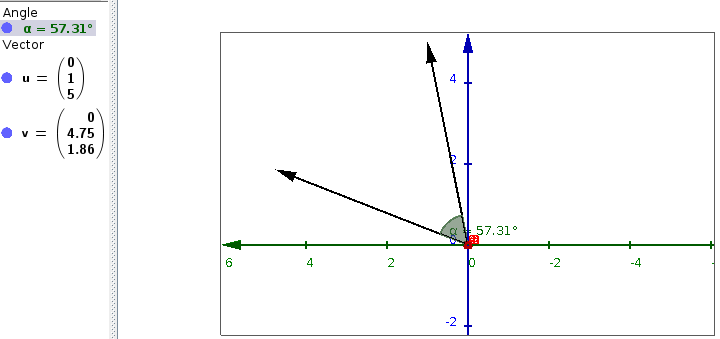
\includegraphics[width=12cm]{rotationsmatrix_eksempel.png}
  \caption{Eksempel på en rotationsmatrix}
  \label{fig:rotationsmatrix_eksempel}
\end{figure}
% Geogebra udregner vinkler i grader, så vi omregner grader til radianer ved hjælp af ligningen:
% \begin{equation}
  % R=d/2*\pi/360=57,31/2*\pi/360\approx1
% \end{equation}
Vi ser at vektor $\vv{u}$ blev drejet \theta radianer, som forventet.


\subsubsection{Konvertering fra farvetemperatur til RGB}
\label{sec:temptilrgb}
Farvetemperatur, som også er beskrevet nederst i \ref{sec:lys}, er temperaturen af et udsendt lys og måles i kelvin. Denne temperatur kan bruges til at finde ud af, om et lys er varmt eller koldt. 
RGB-værdien er en værdi for en given farves indhold af rød, grøn og blå. Værdien angives normalt ved et tal mellem 0 og 255, altså er RBG-værdien [0, 128, 255] ingen del rød, en del grøn og fuld blå, hvilket, blandet sammen, giver en blålig farve.
Der findes ingen direkte og 100\% præcis formel for at ’oversætte’ en kelvintemperaturværdi til en RGB-værdi, derfor har rapporten taget udgangspunkt i en algoritme, som er lavet ud fra 400 målinger, men som stadig ikke er præcis nok til videnskabelig brug \cite{tanner_helland}.
Måden hvorpå algoritmen er lavet, er ved at tage disse 400 målinger, og lave en funktion ud fra dem. Der er lavet én måling per 100 kelvin, der starter ved 1000 kelvin og slutter ved 40.000 kelvin \cite{charity_values}. Ved at kigge på funktionen \cite{tanner_helland_chart} har Tanner Helland kunne konkludere  tre ting:

\begin{itemize}
\item Røde værdier under 6600 kelvin er altid 255.
\item Blå værdier under 2000 kelvin er altid 0.
\item Blå værdier over 6500 kelvin er altid 255.
\end{itemize}

Disse tre, forholdsvis simple, konklusioner har hjulpet med at gøre algoritmen meget kortere og mere simpel. Herunder kan udregningerne for hhv\.  rød-, grøn- og blå-værdierne ses matematisk, før de er skrevet om til kode. Matematikken er vist gennem gaffelfunktioner, altså funktioner med forskellige funktionsudtryk for bestemte intervaller.


\begin{displaymath}
   R(k) = \left\{
     \begin{array}{lr}
       255 &1000 <= \text{k $\land$ k} <= 6600\\
       329.698727446*(k-60^{-0.1332047592}) &6600 < \text{k $\land$ k} <= 40000
     \end{array}
   \right.
\end{displaymath} 

\begin{displaymath}
   G(k) = \left\{
     \begin{array}{lr}
       99.4708025861*\ln(k)-161.1195681661 &1000 <= \text{k $\land$ k} <= 6600\\
       288.1221695283*(k-60^{-0.0755148492}) &6600 < \text{k $\land$ k} <= 40000
     \end{array}
   \right.
\end{displaymath} 

\begin{displaymath}
   B(k) = \left\{
     \begin{array}{lr}
       255 &6600 <= \text{k $\land$ k} <= 40000\\
       0 &1000 <= \text{k $\land$ k} <= 1900\\
       138.5177312231 * \ln(k-10) - 305.0447927307 &1900 < \text{k $\land$ k} < 6600
     \end{array}
   \right.
\end{displaymath} 

Grunden til at der oversættes fra farvetemperatur til RGB-værdi, er for at kunne visualisere farverne på en computer. Et billede vist på en computer består af pixels, som alle har en RGB-værdi, derfor kan lyset fra en lampe med en given farvetemperatur visualiseres, hvis farvetemperaturen oversættes til RGB-værdi.

\paragraph*{Opsummering}
Vi har nu set hvordan man kan konvertere en farvetemperatur i Kelvin til RGB-værdier. Derudover har vi set, hvordan man kan rotere en vektor ved hjælp af matricer. Denne viden er nødvendig for at kunne opfylde kravene om at løsningen skal gøre det muligt at vise lampen med forskellige farvetemperaturer og vinkler. 











\subsubsection{Fra 3D-model til billede}
\label{sec:fra_model_til_billede}
I dette afsnit er formålet nu at vise en model for, hvordan en billeddannelsen af objekter i rummet, også kaldt rendering, kan konstrueres. Dette er essentielt da billeddannelsen danner grundlag for, hvordan 3D-modellen for en lampe omdannes til et billede, der kan vises for kunderne på e-butikken. Til sidst i afsnittet udledes en model for, hvordan belysningen fra en lampe kan simuleres og visualiseres vha. raytracing. 

\paragraph{3D-model}
En 3D-model er en matematisk beskrivelse af et tre dimensionelt objekt. For at beskrive et 3D-objekt opdeler man ofte objektet i trekanter. Dette er illustreret på nedenstående figur.

\begin{figure}[H]
\label{fig:kanin}
    \centering
    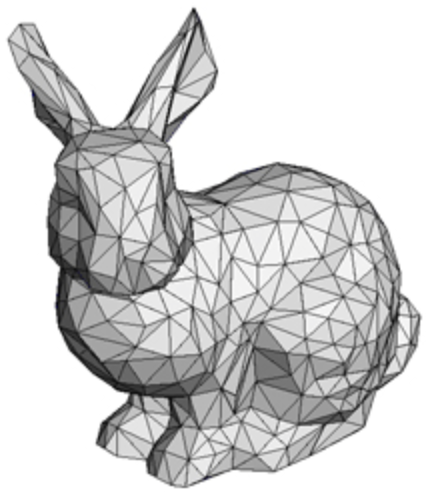
\includegraphics[width=5cm]{kanin}
    \caption{Eksempel hvor trekanter bruges til at repræsentere et objekt: http://www.cs.rpi.edu}
\end{figure}

For at rendere et billede af en 3D-model bestående af trekanter, er man nødt til at have en model for det kamera, som billedet renderes ud fra. Hvordan kameraet kan modelleres er beskrevet i næste afsnit.

\paragraph{Kamera}
Et kamera i konteksten af at rendere en 3D-model, er typisk en beskrivelse af position, orientation og synsfelt. Andre informationer kan tilknyttes som beskriver opløsning af det renderede billede, samt perspektivet af det resulterende billede. Orientationen fastsættes ved hjælp af et sæt vektorer som beskriver hvilken retning der er f.eks.\ højre og op for kameraret.

\begin{figure}[H]
  \centering
  \tdplotsetmaincoords{60}{130}
\begin{tikzpicture}[tdplot_main_coords]
\path[fill=gray!20, draw=gray!40] (-3,-4,-3) -- (-3,-4,3) -- (3,-4,3) -- (3,-4,-3) -- (-3,-4,-3);
\draw (0,0,0) -- (0,-4,0);
\draw[blue!50, thick, -{Stealth[width=2mm, length=2mm]}] (0,0,0) -- (0,-1,0);
\draw[blue!50, thick, -{Stealth[width=2mm, length=3mm]}] (0,-4,0) -- (-1,-4,0);
\draw[blue!50, thick, -{Stealth[width=2mm, length=2mm]}] (0,-4,0) -- (0,-4,1);
\draw[blue!50, thick, -{Stealth[width=2mm, length=2mm]}] (0,0,0) -- (-0.41,-0.8,0.41);
\draw[black, thick, dashed] (-0.41,-0.8,0.41) -- (-2,-4,2);
\draw[black, dashed, thick] (-0,-4,1) -- (-0,-4,2);
\draw[black, dashed, thick] (-0,-4,2) -- (-2,-4,2);
\draw[black, dashed, thick] (-1,-4,0) -- (-2,-4,0);
\draw[black, dashed, thick] (-2,-4,0) -- (-2,-4,2);
\draw plot [mark=*, mark size=2] coordinates{(0,0,0) }; 
\draw plot [mark=*, mark size=2] coordinates{(-2,-4,2) }; 
\node [below] at (0,0,0) {$C$};
\node [below] at (0,-1,-0.1) {$\vv{f}$};
\node [above right] at (0,-2.5,0) {$d$};
\node [above right] at (-2,-4,2) {$B$};
\node [left] at (-2,-4,1) {$y$};
\node [above] at (-1,-4,2) {$x$};
\node [above] at (-1,-4,0) {$\vv{r}$};
\node [right] at (-0.41,-0.8,0.41) {$\vv{s}$};
\node [left] at (0,-4,1) {$\vv{u}$};
\draw[blue!50, thick, |-|] (3.1,-4,3.2) -- (-2.9,-4,3.2);
\draw[blue!50, thick, |-|] (3.2,-4,3.1) -- (3.2,-4,-2.9);
\node [above] at (0,-4,3.2) {$w$};
\node [left]  at (3.2,-4,0) {$h$};
\end{tikzpicture}
  \caption{Visualisering af et punkt på billedplanet som en kombination af tre vektorer $\protect\vv{r}$, $\protect\vv{u}$ og $\protect\vv{f}$, der repræsenterer hhv. højre, op og frem retninger for kameraet.}
  \label{fig:kamera_billede}
\end{figure}

Et punkt $B$ på billedplanet (Se figur \ref{fig:kamera_billede}) kan repræsentere en pixel og kan beskrives som en lineær kombination af en op og en højre orientationsvektor samt en vektor der beskriver afstanden til billedplanet relativt til kammeraet. På figuren er denne vektor $\vv{f}$ skaleret med en faktor $d$.

En stråles retning gennem et pixel koordinat $B$ relativt til kameraets udgangspunkt $C$ kan altså beskrives på følgende måde:
\begin{align}
  \vv{B} &= C + \vv{f} \cdot d + \vv{u} \cdot (y-\frac{h}{2}) + \vv{r} \cdot (x-\frac{w}{2}) \\
  \vv{s} &= \frac{\vv{B}-\vv{C}}{||\vv{B}-\vv{C}||}
\end{align}

Hvor $(x,y)$ er en et koordinat mellem $(0,0)$ og $(w,h)$.

Afstanden $d$ samt størrelsen af billedplanet bestemmer forvrængningen af perspektiv projektionen.

\paragraph{Perspektiv projektion}
\label{sec:perspektiv_projektion}
For at udlede en model for billeddannelsen, tages der udgangspunkt i en perspektiv projektion. Perspektiv projektion er en måde at danne et billede af 3D-objekter ved at projektere objekterne hen på et plan mod et kameras position \cite{perspektive_projection}. Princippet bag perspektiv projektion er vist på figur \ref{fig:perspektiv_projektion}.

\begin{figure}[H]
  \centering
  \tdplotsetmaincoords{60}{130}
\begin{tikzpicture}[tdplot_main_coords]
\path[fill=blue!50, draw=gray!20] (2,-8,2) -- (-2,-8,2) -- (0,-8,0) -- (2,-8,2);
\draw (1,-4,1) -- (2,-8,2);
\draw (-1,-4,1) -- (-2,-8,2);
\draw (0,-4,0) -- (0,-8,0);
\path[fill=gray!20, draw=gray!40] (-2,-4,-2) -- (-2,-4,2) -- (2,-4,2) -- (2,-4,-2) -- (-2,-4,-2);
\path[fill=blue!50, draw=gray!20] (1,-4,1) -- (-1,-4,1) -- (0,-4,0) -- (1,-4,1);
\draw (0,0,0) -- (1,-4,1);
\draw (0,0,0) -- (-1,-4,1);
\draw (0,0,0) -- (0,-4,0);

\draw plot [mark=*, mark size=2] coordinates{(2,-8,2) } ; 
\draw plot [mark=*, mark size=2] coordinates{(-2,-8,2) } ; 
\draw plot [mark=*, mark size=2] coordinates{(0,-8,0) } ; 
\draw plot [mark=*, mark size=2] coordinates{(1,-4,1) }; 
\draw plot [mark=*, mark size=2] coordinates{(-1,-4,1) }; 
\draw plot [mark=*, mark size=2] coordinates{(0,-4,0) }; 
\draw plot [mark=*, mark size=2] coordinates{(0,0,0) }; 
\node [above left] at (2,-8,2) {$P$};
\node [above left] at (1,-4,1) {$B$};
\node [above right] at (0,0,0) {$C$};
\end{tikzpicture}
  \caption{Viser princippet bag perspektiv projektion af et punkt på et billedplan.}
  \label{fig:perspektiv_projektion}
\end{figure}

Som vist på figur \ref{fig:perspektiv_projektion} kan et punkt $P\in \mathbb{R}^3$ projekteres ned på billedplanen $\alpha$ ved at finde skæringspunktet $B$ mellem billedplanen $\alpha$ og en lysstråle $L$, som går fra punktet $P$ mod kameraets position $C$. Gør man nu dette for alle punkter på et objekt i rummet, og tegner skæringspunkterne på billedplanen, dannes et billede af objektet, ved at oversætte punktet på billedplanen, til (x,y)-pixelkoordinater, på det resulterende billede, med udtrykket beskrevet under afsnittet om kameraet.

Udfordringen er så at afgøre hvilken farve punkterne på billedplanen skal have, da dette afhænger af objektets egenskaber, samt hvilket udefrakommende lys der rammer objektet. 

For at løse denne udfordring, benytter vi i dette projekt raytracing, der som beskrevet under afsnit \ref{sec:computergrafik}, bygger på at simulere lysstrålers interaktion med forskellige objekter i rummet. Hvordan dette fungere er beskrevet i næste afsnit, hvor der er beskrevet en model for backwards raytracing.

\paragraph{Backwards raytracing}
I modsætning til en perspektiv projektion af et punkt på et plan, er backwards raytracing, hvor man i stedet for punktet i rummet, tager udgangspunkt i de lysstråler der danner billedet. Ved backwards raytracing følger man lysstrålerne baglæns og ser på, hvor stor en lysintensitet, den pågældende lysstråle har efter den har interageret med objekterne i rummet. Ud fra dette farves det tilhørende punkt på billedet, og på den måde kan man rendere et helt billede. På figur \ref{fig:raytracing_skitse} er det vist hvordan man kan konstruere en lysstråle ud fra et bestemt punkt på billedplanen, hvor lysstrålen er beskrevet ved en retningsvektor og et startpunkt.

\begin{figure}[H]
  \centering
  \tdplotsetmaincoords{60}{130}
  \begin{tikzpicture}[tdplot_main_coords]
  \path[fill=blue!50, draw=gray!20] (2,-8,2) -- (-2,-8,2) -- (0,-8,0) -- (2,-8,2);
\draw (0,0,0) -- (0,-8,1);
\path[fill=gray!20, draw=gray!40] (-2,-4,-2) -- (-2,-4,2) -- (2,-4,2) -- (2,-4,-2) -- (-2,-4,-2);
\draw plot [mark=*, mark size=2] coordinates{(0,-4,0.5) }; 
\draw plot [mark=*, mark size=2] coordinates{(0,0,0) }; 
\node [above right] at (0,-4,0.5) {$B$};
\node [above right] at (0,0,0) {$C$};
\draw [blue!50, thick, -{Stealth[width=3mm, length=3mm]}] (0,0,0) -- (0,-4,0.5);
\node [above right] at (0,-2,0.25) {$\vv{r}$};
\end{tikzpicture}
  \caption{Viser hvordan en der kan opstilles retningsvektor mellem kameraets position $C$ og punktet $P$ på billedplanen, som sammen med startpunktet $C$ beskriver lysstrålen fra trekanten i omvendt retning.}
  \label{fig:raytracing_skitse}
\end{figure}

Retningsvektoren $\vv{r}$ for lysstrålen kan heraf beskrives som følgende.

$$ \vv{r} = \vv{B} - \vv{C} $$

Hvor $\vv{B}$ og $\vv{C}$ er stedvektorer for hhv. punktet på billedplanen $B$ og kameraets position $C$.

Lysstrålen kan på den måde beskrives ved følgende vektorfunktion.

$$ \vv{l}(t) = \vv{r} t + \vv{C}$$

Hvor $t$ er en skalar i $\mathbb{R}$.

For at finde ud af hvilken farve punktet på billedplanen $B$ skal have, ser man hvordan lysstrålen rammer de forskellige objekter der skal renderes.

Der findes flere forskellige modeller for hvordan lysintensiteten for en lysstråle beregnes. En simpel model, er Phong-modellen, som opdeler lys i forskellige kategorier: ambient, diffuse og specular.

\paragraph{Phong-modellen}
Phong-modellen er en såkaldt \textit{shading} funktion, som beskriver lyset fra punkter på et objekt på baggrund af lyskilden, objektet og kameraets synsvinkel\cite{phong_paper}. Der findes flere forskellige variationer af phong-modellen. Da vi som vist i afsnit \ref{sec:temptilrgb} kan arbejde med farvetemperaturer via rgb-værdier, så har vi valgt en variation af phong-modellen, som beskriver lys via rgb-værdier. 

Ud fra modellen\cite{stanford_phong}, kan der skrives følgende overordnede \textit{shading} funktion.
\begin{equation} \label{eq:phong}
  \rho = \rho_a + \sum\limits_{lights} (\rho_d + \rho_s)
\end{equation}
Hvor $\rho_a$, $\rho_l$ og $\rho_s$ er hhv. \textit{ambient}, \textit{diffuse} og \textit{specular} lys der er beskrevet kort herunder.

\subparagraph{\textit{Ambient} lys} repræsenterer det lys, som reflekteres rundt i rummet og rammer objekter ligeligt fra alle sider\cite{stanford_phong}. Formlen til at beregne dette er følgende\cite{stanford_phong}.
\begin{align}
\label{eq:ambient_formel}
	\rho_a &= m_a C A
\end{align}
Hvor $m_a$ er den ambiente konstant, $C$ er overfladens farve som rgb-værdi og $A$ er den ambiente lysintensitet.

\subparagraph{\textit{Diffuse} lys} er det lys, som reflekteres ifølge \textit{Lambert's Cosinuslov}. Ud fra loven kan følgende model anvendes til at udregne \textit{diffuse} lys\cite{stanford_phong}.
\begin{align}
	\rho_l &= m_l C I max(\vv{I}\bullet\vv{n}, 0)
\end{align}
Hvor $m_l$ er den Lambertianske konstant, $I$ er det lyskildens lysintensitet, $\vv{I}$ og $\vv{n}$, er normaliserede vektorer, hhv. vektor fra overfladepunktet mod lyskilden og normalvektoren til overfladepunktet.

\subparagraph{\textit{Specular} lys} er det lys der spejles i objektets overflade, givet ved nedenstående formel\cite{stanford_phong}.
\begin{align}
	\rho_s &= m_s S I max(\vv{r}\bullet\vv{u},0)^{m_{sp}} \\
	S &= m_{sm} C + (1 - m_{sm})(1,1,1)
\end{align}
Hvor $m_s$ er den specular konstant, $S$ er en lineær interpolation mellem objektets farve og hvid, afhængig af objektets \textit{metalness} $m_{sm}$. $\vv{u}$ og $\vv{r}$ er normaliserede vektorer, for hhv. vektor fra overfladepunktet mod kameraet og retningsvektor for det reflekterede lys beregnet som følgende.
\begin{align}
	\vv{r} &= -\vv{I} + 2 (\vv{I} \bullet \vv{n}) \vv{n}
\end{align}

De anvendte vektorer til phong \textit{shading} funktionen er vist på figuren herunder.
\begin{figure}[H]
  \label{fig:phong_skitse}
  \centering
  \tdplotsetmaincoords{60}{130}
  \begin{tikzpicture}[tdplot_main_coords]
  \draw plot [mark=*, mark size=2] coordinates{(0,-4,2) }; 
\node [above left] at (0,-4,2) {$C$};
  \draw (0,-4,2) -- (0,-3,1.5);
  \path[fill=gray!20, draw=gray!40] (-1,-3,1) -- (-1,-3,3) -- (1,-3,3) -- (1,-3,1);

  \path[fill=gray!20, draw=gray!40] (1,-2,0) -- (-1,0,0) -- (1,2,0);
    \draw (0,-3,1.5) -- (0,0,0);
    \draw [blue!50, thick, -{Stealth[width=3mm, length=3mm]}] (0,0,0) -- (0,0,2.24);
    \node [above] at (0,0,2.24) {$\vv{n}$};
    \draw [blue!50, thick, -{Stealth[width=3mm, length=3mm]}] (0,0,0) -- (0,-2,1);
    \node [below left] at (0,-2,1) {$\vv{u}$};
    \draw [blue!50, thick, -{Stealth[width=3mm, length=3mm]}] (0,0,0) -- (0,-1,2);
    \node [above left] at (0,-1,2) {$\vv{r}$};
    \draw (0,0,0) -- (0,2,4);
    \draw plot [mark=*, mark size=2] coordinates{(0,2,4) }; 
    \node [above right] at (0,2,4) {$L$};
    \draw [blue!50, thick, -{Stealth[width=3mm, length=3mm]}] (0,0,0) -- (0,1,2);
    \node [right] at (0,1,2) {$\vv{I}$};
 \draw (0,0.3, 1.1) -- (0,0.35, 1.3);
  \draw (0,0.35, 1.1) -- (0,0.4, 1.3);
  
 \draw (0,-0.2, 0.9) -- (0,-0.25, 1.1);
  \draw (0,-0.15, 0.95) -- (0,-0.2, 1.15);

  \draw (0,-1,2) coordinate (a)
  (0,0,0) coordinate (b)
  (0,0,2.24) coordinate (c)
  pic[draw=black,|-|,angle eccentricity=1.2,angle radius=1cm] {angle=c--b--a};
  \draw (0,0,2.24) coordinate (a)
  (0,0,0) coordinate (b)
  (0,1,2) coordinate (c)
  pic[draw=black,|-|,angle eccentricity=1.2,angle radius=1cm] {angle=c--b--a};
\draw plot [mark=*, mark size=2] coordinates{(0,0,0) }; 
    \node [below right] at (0,2,4) {$P$};
\end{tikzpicture}
  \caption{Viser vektorer der anvendes i phong-modellen. $\protect\vv{u}$ er vektor mod kameraet med position $C$, $\protect\vv{n}$ er normalvektoren til objektet i punktet $P$, $\protect\vv{I}$ er vektor mod lyskildens position $L$ og $\protect\vv{r}$ er vektor for det reflekterede lys.}
\end{figure}

\subsubsection{Skæring mellem linje og trekant i rummet}
\label{sec:triangle_intersection}
For at finde om der er en skæring mellem en stråle og en trekant, kan man følge tre trin:
\begin{enumerate}
  \item Find skæringen med trekantens plan og påvis at punktet er foran strålens udgangspunkt
  \item Påvis at punktet i trekantens plan, ligger indenfor trekanten
  \item Påvis at strålens linje ikke er parallel med trekantens plan
\end{enumerate}

En stråle er paralel med et plan hvis strålens retning er 90 grader relativt til planets normalvektor, dette er sandt hvis ligning \ref{eq:parralel} er opfyldt.

\begin{equation}
  \label{eq:parralel}
  \vv{r} \bullet \vv{n} = 0
\end{equation}

Planets normalvektor findes ved at krydse to vektore fra en af trekantens hjørner til de to andre (se ligning \ref{eq:triangle_normal}).

\begin{equation}
  \label{eq:triangle_normal}
  \vv{n} = (B - A) \times (C - A)
\end{equation}

\begin{figure}[H]
  \centering
  \tdplotsetmaincoords{60}{130}
  \begin{tikzpicture}[tdplot_main_coords]
    % dashed line through plane
    \draw [black, thick] (0,0,0) -- (4,-8,4);
    % triangle and plane
    \path[fill=gray!10, draw=gray!20] (0,-4,0) -- (4,-4,0) -- (4,-4,4) -- (0,-4,4) -- (0,-4,0);
    \path[fill=gray!30, draw=gray!60] (1,-4,2) -- (2,-4,3) -- (3,-4,1) -- (1,-4,2);
    % triangle
    \draw [blue!50, thick, -{Stealth[width=3mm, length=3mm]}] (2,-4,3) -- (3,-4,1);
    \draw [blue!50, thick, -{Stealth[width=3mm, length=3mm]}] (2,-4,3) -- (1,-4,2);
    \draw [blue!50, thick, -{Stealth[width=3mm, length=3mm]}] (2,-4,3) -- (2,-2,3);
    % \draw [black,   thick, -{Stealth[width=2mm, length=2mm]}] (2,-4,3) -- (2,-4,2);
    \node [above] at (2,-3,3) {$\vv{n}$};
    \node [above] at (2,-4,3) {$A$};
    \draw plot [mark=*, mark size=1] coordinates{(2,-4,3) }; 
    \node [left] at (3,-4,1) {$B$};
    \draw plot [mark=*, mark size=1] coordinates{(3,-4,1) }; 
    \node [below] at (1,-4,2) {$C$};
    \draw plot [mark=*, mark size=1] coordinates{(1,-4,2) };
    
    % ray
    \node [above right] at (0,0,0) {$P_0$};
    \draw plot [mark=*, mark size=1] coordinates{(0,0,0) };
    \node [above right] at (0.25,-0.5,0.25) {$\vv{r}$};
    \draw [black, thick] (0,0,0) -- (2,-4,2);
    \draw [blue!50, thick, |-|] (0.1,0,-0.1) -- (2.1,-4,1.9);
    \node [below left] at (1,-2,1) {$t_A$};
    \node [black, above left] at (2.5,-4,2) {$P(t_A)$};
    \draw [black, thick, -{Stealth[width=3mm, length=3mm]}] (0,0,0) -- (0.5,-1,0.5);
    \draw plot [mark=*, mark size=1] coordinates{(2,-4,2) };
  \end{tikzpicture}
  \caption{Viser princippet bag perspektiv projektion af et punkt på et billedplan.}
  \label{fig:perspektiv_projektion}
\end{figure}

Hvis strålen ikke er parralel med planet kan vi nu finde et punkt i planet som strålen skære. Alle vektore i planet er ortogonale på normal vektoren, dermed kan vi opstille ligning \ref{eq:vektor_in_plane} til at beskrive betingelsen for et punkt strålen som også ligger i planet. Ved at substituere linjens ligning (ligning \ref{eq:point_on_ray}) ind og isolere $t_A$ kan vi så bruge til at finde punktet på strålens linje og er $t_A > 0$ så er punktet også foran strålens udgangspunkt $P_0$

\begin{align}
  \label{eq:point_on_ray}
  P(t) &= \vv{r} \cdotp t + \vv{P_0} \\
  \label{eq:vektor_in_plane}
  ( P(t_A) - A ) \bullet \vv{n} &= 0 \\
  \label{eq:test3}
  (\vv{r} \cdotp t_A + \vv{P_0} - A) \bullet \vv{n} &= 0 \\
  \label{eq:test4}
  t_A \cdotp \vv{r} \bullet \vv{n} + (\vv{P_0} - A) \bullet \vv{n} &= 0 \\
  \label{eq:test5}
  t_A &= -\frac{(\vv{A} - \vv{P_0})\bullet \vv{n}}{\vv{r} \bullet \vv{n}}
\end{align}


[FIND IF POINT IS INSIDE TRIANGLE]()

\begin{figure}[H]
  \centering
  \tdplotsetmaincoords{60}{130}
  \begin{tikzpicture}[tdplot_main_coords,thick,scale=2, every node/.style={transform shape}]
    \coordinate (Pt) at (2,-4,2);
    \coordinate (A) at (2,-4,3);
    \coordinate (B) at (3,-4,1);
    \coordinate (C) at (1,-4,2);
    % dashed line through plane
    % triangle and plane
    \path[fill=gray!10, draw=gray!20] (0.8,-4,0.8) -- (3.2,-4,0.8) -- (3.2,-4,3.2) -- (0.8,-4,3.2) -- (0.8,-4,0.8);
    \path[fill=gray!30, draw=gray!60] (A) -- (B) -- (C) -- (A);
    % triangle
    \draw [blue!50, thick, -{Stealth[width=3mm, length=3mm]}] (A) -- (B);
    \draw [blue!50, thick, -{Stealth[width=2mm, length=2mm]}] (A) -- (Pt);
    \draw [blue!50, thick, -{Stealth[width=3mm, length=3mm]}] (B) -- (C);
    \draw [blue!50, thick, -{Stealth[width=2mm, length=2mm]}] (B) -- (Pt);
    \draw [blue!50, thick, -{Stealth[width=3mm, length=3mm]}] (C) -- (A);
    \draw [blue!50, thick, -{Stealth[width=2mm, length=2mm]}] (C) -- (Pt);
    \node [above] at (2,-3,3) {$\vv{n}$};
    \node [above] at (2,-4,3) {$A$};
    \draw plot [mark=*, mark size=1] coordinates{(2,-4,3) }; 
    \node [left] at (3,-4,1) {$B$};
    \draw plot [mark=*, mark size=1] coordinates{(3,-4,1) }; 
    \node [below] at (1,-4,2) {$C$};
    \draw plot [mark=*, mark size=1] coordinates{(1,-4,2) };
    
    % ray
    \node [black, above left] at (2.5,-4,2) {$P(t_A)$};
    \draw plot [mark=*, mark size=1] coordinates{(2,-4,2) };
  \end{tikzpicture}
  \caption{Viser princippet bag perspektiv projektion af et punkt på et billedplan.}
  \label{fig:perspektiv_projektion}
\end{figure}


\subsubsection{Kd-træer}
\label{sec:kdtree}

Kd-træer er binære træer, hvilket betyder at hver node maksimalt har to under-noder. K'et i kd-træ er antallet af dimensioner, men i stedet for 3D træ, siger man et 3-dimensionelt kd-træ. Kd-træer bruges til at minimere antallet af søgninger, som et givent program skal gennemføre. 

Et kd-træ opbygges ved at have en mængde af værdier, som er usorterede. Disse værdier kan inddeles i et træ, ved at finde et taktisk splittepunkt, som er roden. Herefter går to noder ud fra roden, den venstre har den nedre halvdel af værdierne og den højre har den øvre halvdel. Herefter splittes disse to noder hver for sig igen, og sådan fortsætter træet indtil fastsatte krav nås, hvorefter man så kalder den sidste række af noder for bladene. 

En simpel forklaring af et to-dimensionelt kd-træ kan være et program til at finde tallet 100 i en tilfældig mængde fra 1-1000. Roden deles på et bestemt punkt, hvilket i dette tilfælde er midtpå ved 500, og derfor vil den venstre under-node til 'rod-noden' indeholde værdier, der er lig med eller under 500 og det højre barn til indeholde værdier, der er højere end eller lig med 500. Sådan fortsætter programmet med at halvere alle muligheder efter hvert niveau indtil den ønskede værdi er fundet. Denne metode kræver i teorien færre sammenligninger og bør dermed være hurtigerer for store datasæt end hvis man bad et program om at finde et givent tal mellem 1 og 1000, da den, i værste tilfælde, skulle tjekke 999 tal igennem, før den fandt det ønskede nummer.

\begin{figure}[H]
  \centering
  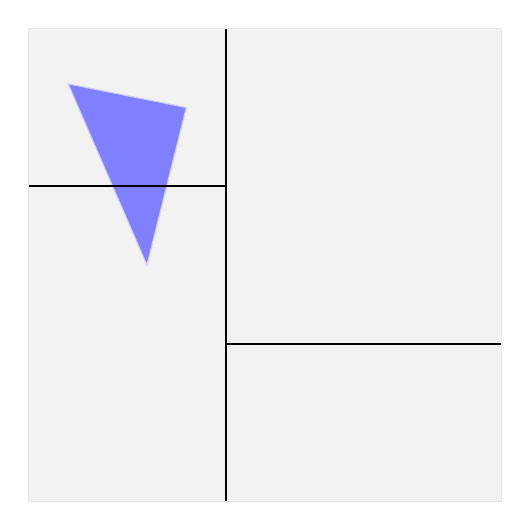
\begin{tikzpicture}
    \path[fill=gray!10, draw=gray!20] (3,3) -- (3,-3) -- (-3,-3) -- (-3,3) -- (3,3);
    
    \path[fill=blue!50, draw=blue!20] (-1,2) -- (-2.5,2.3) -- (-1.5,0) -- (-1,2);
    
    \draw [black, thick] (-0.5, -3) -- (-0.5, 3);
    \draw [black, thick] (-0.5, -1) -- ( 3,  -1);
    \draw [black, thick] (-0.5,  1) -- (-3,   1);
    % triangle
    % \draw [blue!50, thick, -{Stealth[width=3mm, length=3mm]}] (2,-4,3) -- (3,-4,1);
    % \draw [blue!50, thick, -{Stealth[width=3mm, length=3mm]}] (2,-4,3) -- (1,-4,2);
    % \draw [blue!50, thick, -{Stealth[width=3mm, length=3mm]}] (2,-4,3) -- (2,-2,3);
    % \draw [black,   thick, -{Stealth[width=2mm, length=2mm]}] (2,-4,3) -- (2,-4,2);
    % \node [above] at (2,-3,3) {$\vv{n}$};
    % \node [above] at (2,-4,3) {$A$};
    % \draw plot [mark=*, mark size=1] coordinates{(2,-4,3) }; 
    % \node [left] at (3,-4,1) {$B$};
    % \draw plot [mark=*, mark size=1] coordinates{(3,-4,1) }; 
    % \node [below] at (1,-4,2) {$C$};
    % \draw plot [mark=*, mark size=1] coordinates{(1,-4,2) };
    
    % ray
    % \node [above right] at (0,0,0) {$P_0$};
    % \draw plot [mark=*, mark size=1] coordinates{(0,0,0) };
    % \node [above right] at (0.25,-0.5,0.25) {$\vv{r}$};
    % \draw [black, thick] (0,0,0) -- (2,-4,2);
    % \draw [blue!50, thick, |-|] (0.1,0,-0.1) -- (2.1,-4,1.9);
    % \node [below left] at (1,-2,1) {$t_A$};
    % \node [black, above left] at (2.5,-4,2) {$P(t_A)$};
    % \draw [black, thick, -{Stealth[width=3mm, length=3mm]}] (0,0,0) -- (0.5,-1,0.5);
    % \draw plot [mark=*, mark size=1] coordinates{(2,-4,2) };
  \end{tikzpicture}
  \caption{KD-træ}
  \label{fig:kd-tree}
\end{figure}
---
% \begin{figure}[H]
%   \centering
%   \begin{tikzpicture}[
%     level 1/.style={sibling distance=40mm},
%     level 3/.style={sibling distance=20mm},
%     level 4/.style={sibling distance=10mm},
%     every node/.style={draw,circle},
%     arrow/.style={edge from parent/.style={draw,-latex}}
%   ]
%   \node {A}
%     child { node{B}
%       child { node{D}
%         child {node{H}}
%         child {node{I}}
%       }
%       child { node{E}
%         child {node{J}}
%         child {node{K}}
%       }
%     }
%     child { node{C}
%       child { node{F}
%         child {node{L}}
%         child {node{M}}
%       }
%       child { node{G}
%         child {node{N}}
%         child {node{O}}
%       }
%     }
%   ;
%   \end{tikzpicture}
%   \caption{KD-træ}
%   \label{fig:kd-tree}
% \end{figure}

\subsubsection*{Opsummering}

Ud fra teoridiskussionen kan der nu kortfattets hvordan teorierne bidrager til programudviklingen. 

Rotationsmatricer giver den empiri som skal til for at roterer vektorer i rummet med en vilkårlig vinkel. Dette er relevant når man skal flytte kameraets position, som hører til programkravet om at lampens belysning skal kunne visualiseres fra flere forskellige vinkler.

Teorien om konvertering fra farvetemperatur til RGB giver os den algoritme som skal til for, at lave en farvetemperatur i kelvin om til en RGB-værdi. Dette er relevant i forhold til programkravet om at kunne ændre pærens farvetemperatur. 

Teorien fra 3D-model til billede omhandler matematiske modeller og beskrivelser af relevante teknologier og algoritmer. Teorien i dette er relevant for, at forstå nogle af grundprincipperne i en raytracer heriblandt backwards raytracing og Phong-modellen.

Teorien om ray-triangle intersection omhandler en matematisk model over, hvordan man finder skæringen mellem en ray og en trekant i planen. Dette knytter sig til teorien om en 3D-model, da alle objekter består af trekanter. 

Som afslutning på teoridiskussionen opstilles følgende nye krav til programudviklingen i forhold til kravene i afsnit \ref{sec:krav}:
\begin{enumerate}
    \item Programmet skal kunne modtage følgende input fra brugeren: 3D-fil af lampen og dens kontekst, billedets opløsning, pærens farvetemperatur og hvilken synsvinkel man ønsker at se billedet fra (kameraets position).
    \item Programmet skal ved brug af raytracing kunne fremstille et billede af lampen og dens belysning på baggrund af brugerinputtet. Derudover skal raytracerens renderingstid optimeres ved brug af KD-træer.
    \item Programmet skal kunne gemme det renderede billede.
\end{enumerate}